% web10 paper: text revision for the SIGMOD 2027 industry target
% Render: tectonic main.tex  (from this directory)
\documentclass[sigconf, nonacm, review]{acmart}

% --- packages (all in the tectonic bundle) ---
\usepackage{booktabs}
\usepackage{enumitem}
\usepackage{microtype}
\usepackage{xcolor}
\usepackage{listings}
\usepackage{graphicx}

\lstdefinestyle{sql}{
  language={},
  basicstyle=\ttfamily\footnotesize,
  breaklines=true,
  frame=single,
  framesep=4pt,
  rulecolor=\color{gray!50},
  backgroundcolor=\color{gray!6},
  keywordstyle=\bfseries,
}
\lstdefinestyle{json}{
  language={},
  basicstyle=\ttfamily\footnotesize,
  breaklines=true,
  frame=single,
  framesep=4pt,
  rulecolor=\color{gray!50},
  backgroundcolor=\color{gray!6},
}

% --- acmart metadata ---
\setcopyright{none}
\acmConference[SIGMOD 2027 Industry Track (Target)]{Draft targeting the SIGMOD 2027 Industry Track}{}{}
\acmPrice{}
\acmISBN{}
\acmDOI{}

\title{Your Data, Your Rules: \\ Query-Layer Access for a Social Data Platform}
\author{Jacob Hoffman}
\affiliation{\institution{web10 Inc.}\country{}}
\email{jacob@web10.app}

\begin{document}

\begin{abstract}
Social applications typically implement content, audience relationships, and
access rules in application-specific backends. \textbf{web10} places content
and access relationships in a shared data platform, allowing applications to
define their own queries while users manage group membership and grants. The
platform stores documents under logical user namespaces in ClickHouse and
exposes generic groups, service-scoped roles, app contracts, and a query API.
Its central mechanism is a query boundary: application queries name services,
and the node supplies filtered relations for the reader before executing joins
and aggregations. A deployed social application uses this mechanism to combine
ranked posts, engagement, and profiles, with media capabilities prepared by the
node. We describe the access model, query compilation, and application
composition, including the costs of metadata resolution and the consistency
obligations of a shared columnar store. The design separates application-defined
social queries from shared access enforcement. This draft specifies the
feasibility evaluation; latency, capacity, revocation, and cost results remain
pending.
\end{abstract}

\maketitle

%=============================================================================
\section{Introduction}
\label{sec:intro}

For a creator, an audience is more than a list of accounts. It is a set of
relationships: who follows, who belongs to a group, and who may read or contribute
content. When those relationships live inside one application's backend, a new
frontend must recover both the data and the rules that give it meaning. The
database question is how to make content and access relationships reusable
across applications while preserving the reader's authorization boundary.

\textbf{web10} addresses this question with a shared data plane and a small set
of composable access primitives. A user's key identifies a logical namespace,
not a separate database. Generic groups associate documents with audiences;
roles name per-service operations; app contracts constrain supported calling
contexts. An application supplies its own services and queries rather than
requiring a new feed endpoint for each ranking or audience model.

The motivating application is a deployed creator-oriented social platform,
including feeds, groups, direct messages, discovery, and monetization. Its feed
illustrates the separation: an application chooses chronological or weighted
ranking, while the node resolves the reader's access. A chronological query
makes eligible posts retrievable without an engagement-based cutoff, subject
to access and moderation rules. Here distribution means eligibility for
retrieval; pagination and user attention determine what is actually viewed.

This work builds on the decentralized social web. ActivityPub defines activity
delivery APIs~\cite{activitypub2018}; ATProto separates repositories, relays,
and application views~\cite{kleppmann2024}; Solid separates applications from
personal data stores~\cite{solid2016}. Solid's Web Access Control supports group
agents~\cite{wac2022}, and its Access Control Policy includes a client
dimension~\cite{acp2022}. web10 brings user-facing contracts and application-written
SQL together within one node's shared columnar store. This placement lets an
application compose cross-service reads against relations filtered for its
reader, rather than define a dedicated server endpoint for each social view.

We use \emph{generic social composition} to mean that app-defined content and
relationships are represented through service-namespaced documents, generic
group membership, role maps, and queries. Generic group-management endpoints
are part of this substrate. The node also provides advertising, content-event,
media, and result-preparation machinery. The architectural separation is between
application-defined content and query semantics and these shared node services.

This paper makes three contributions:

\begin{enumerate}[leftmargin=*,nosep]
  \item \textbf{A compositional data/access architecture}
  (\S\ref{sec:model}): logical user namespaces, app contracts, and group roles
  share a service-scoped permission vocabulary, exposed to application authors
  and users rather than only infrastructure operators.
  \item \textbf{A reader-specific query boundary}
  (\S\ref{sec:enforcement}): service references resolve to filtered CTEs before
  caller joins and aggregation. The implementation combines policy resolution,
  SQL validation, and boundary construction above a shared database account.
  \item \textbf{A deployed social application case study}
  (\S\ref{sec:eval}): ranked feeds combine content, engagement, profiles, and
  media through application queries and node preparation. The case study shows
  how access scope shapes query results and follow-up reads.
\end{enumerate}

The evaluation in \S\ref{sec:method} will assess practical operating points
and characterize the architecture's costs. This submission's goal is feasibility
and a clear account of tradeoffs; further optimization is follow-up work.
Measurements remain pending in this draft.
\S\ref{sec:related} relates the design to decentralized storage, IAM, and
multi-tenant databases; \S\ref{sec:concl} concludes.

%=============================================================================
\section{The Access Model}
\label{sec:model}

\subsection{Two trust layers}

For a group-scoped content operation, the model distinguishes an \emph{app}, a
\emph{principal} (the acting user), a \emph{group} $G$, a \emph{service} $S$
(a data namespace such as \texttt{posts} or \texttt{comments}), and an
\emph{operation} $O$ (e.g.\ \texttt{readAll}, \texttt{create}). Authorization
asks two questions where the corresponding gates apply:

\begin{center}
\small
\resizebox{\columnwidth}{!}{%
\begin{tabular}{@{}ll@{}}
\toprule
\textbf{Layer} & \textbf{Question} \\
\midrule
App trust (outer wall)   & Can this \emph{app} perform $O$ on $S$? \\
Person trust (inner wall) & Does membership or a class/role grant allow $O$ on $S$ in $G$? \\
\bottomrule
\end{tabular}}
\end{center}

The app contract expresses trust in a calling application. In the current
document and query paths, authenticated browser-style tokens are checked against
an origin-keyed contract when an HTTP \texttt{Origin} is present; without that
header, this app-contract check is skipped. Anonymous queries also skip it.
OAuth-delegated tokens instead select a \texttt{client\_id}-keyed contract,
including when no Origin is present. The node enables wildcard, non-credentialed
CORS; endpoint code enforces application grants separately. CORS is not
cryptographic client authentication and does not constrain a non-browser
client's choice of headers. Thus the outer layer is not a universal gate on
every API call. Identity verification and document/group authorization remain
distinct from this calling-context policy.

The group layer expresses trust in people. The split lets a user revoke an
app grant without leaving a group, or leave a group without changing app
grants. Describing this policy decomposition does not certify all issuance,
consent, and delegation paths (\S\ref{sec:method}).

\subsection{Roles are per-service permission maps}

A role is a named bundle of per-service permissions---a map from service to
the operations it grants:

\begin{lstlisting}[style=json]
{ "name": "editor",
  "permissions": {
    "posts":    ["readAll", "create", "updateOwn"],
    "comments": ["readAll"]
  } }
\end{lstlisting}

The map \emph{is} the scope. \texttt{'*'} wildcards all document services; a
reserved key \texttt{'group'} carries \emph{structural} operations on the
group itself (\texttt{manageRoles}, \texttt{assignRoles},
\texttt{deleteGroup}, join/member operations), while \emph{content}
operations---including moderation such as \texttt{hideAll}---live under the
service key, because they act on documents, not on the group's shape.

Two properties keep the model small. First, the role map is the
\emph{same shape} as the app-contract permission object: there is one
permission language across both trust layers. Second, a person holds
\emph{one explicit member role} per group; compound permissions can be placed
in that role rather than stacked through multiple assignments. This positive
grant model does not express every policy, such as explicit deny or arbitrary
context-dependent conditions. Roles are generic---a group defines
whatever roles fit its purpose (\texttt{owner}, \texttt{moderator},
\texttt{page-curator}, \texttt{member}, or \texttt{dj}, \texttt{listener})---
and applications supply their role definitions. Some lifecycle operations use
conventional names such as \texttt{member}; the extensibility claim is not that
every role name is unknown to the implementation.

\subsection{Principal classes and effective permissions}

Access is granted to \emph{principals}, of which there are three nested
classes, broadest to narrowest:

\begin{center}
\small
\begin{tabular}{ll}
\toprule
\textbf{Class} & \textbf{Who} \\
\midrule
\texttt{anyone}        & every request, signed in or not \\
\texttt{authenticated} & a verified non-anonymous user, member or not \\
\texttt{member}        & holds a member row in this group \\
\bottomrule
\end{tabular}
\end{center}

The broad classes \texttt{anyone} and \texttt{authenticated} are represented by
\emph{reserved keys in the member table}; individual members use their own
principal keys. No separate visibility table is needed. For example:

\begin{lstlisting}[style=sql]
group_members:
  (G, 'anyone',        'reader')    -- the group is public
  (G, 'authenticated', 'reader')    -- signed-in users can read
  (G, 'bob',           'moderator') -- bob moderates
  (G, 'alice',         'owner')     -- alice owns
\end{lstlisting}

A principal's \emph{effective} permissions in a group are the union of the
permission maps of every class they belong to:

\begin{center}
\small
$\mathrm{effective}(P, G) \;=\; \mathrm{grant}(G,\ \texttt{anyone})$\\
$\quad \cup\ \big(P \in \texttt{authenticated} \;?\; \mathrm{grant}(G,\ \texttt{authenticated}) : \emptyset\big)$\\
$\quad \cup\ \big(P \in \texttt{member}(G) \;?\; \mathrm{grant}(G,\ \mathrm{role}(P)) : \emptyset\big)$
\end{center}

This equation describes the union of explicit grants, not the whole current
content gate. In the implemented \texttt{can\_read\_group} and
\texttt{can\_write\_group} helpers, an active member is admitted for content
reads and creates without requiring service-specific \texttt{readAll} or
\texttt{create} in that member's role. For non-members, the class grants supply
those permissions. Other role-controlled operations still require their own
checks. In particular, omitting \texttt{readAll} from a member role is not a
way to hide that service from the member in these paths.

The union is monotone across principal classes under otherwise equal
conditions. Actual visibility also depends on blocks, sharing state, hidden
documents, and node moderation; the equation alone is not a theorem that every
member sees a superset of every stranger's results.

\subsection{Publicness is a grant, not a flag}

There is no \texttt{visibility} column. ``Make my group public'' is the act
of granting \texttt{readAll} to \texttt{anyone}; ``signed-in only'' grants it
to \texttt{authenticated}; ``private'' withholds those non-member grants. Join
policy is orthogonal: it controls how a human \emph{becomes} a member (open,
request, invite-only) and says nothing about what a non-member bystander can
see. A group can be invite-only to join and still publicly readable---the
discovery board is exactly that.

This is the sense in which web10 brings IAM to the front: the operations a
cloud operator would express as policies---\emph{principal class, service,
operation, grant}---are the operations an \emph{end user} expresses about
their own data. A grant is represented by metadata rows and revoked through
tombstones. Subsequent checks use latest-row resolution, but an end-to-end
revocation bound must also account for concurrent checks, database visibility,
and already issued capabilities; it is not established merely by writing a
tombstone.

%=============================================================================
\section{Enforcement at the Query Layer}
\label{sec:enforcement}

\subsection{One columnar table}

A ranked feed has analytical components: joins across authors and engagement,
filtering, aggregation, and sorting. A social application also has point reads,
updates, and coordination-heavy operations; calling the entire workload OLAP
would conceal that mixture. web10 chooses ClickHouse~\cite{clickhouse2024} for
both structured content and operational metadata rather than maintaining a
separate Postgres-to-ClickHouse replication pipeline. User content occupies
one shared \texttt{documents} table keyed by \texttt{(author\_key, doc\_id)}.
The user namespace is logical isolation within that table, not a per-user
database or physical collection. Large media objects reside in object storage.
The following simplified schema omits reference and advertising fields:

\begin{center}
\begin{minipage}{\columnwidth}
\begin{lstlisting}[style=sql]
CREATE TABLE documents (
    doc_id          String,
    author_key      String,
    collection_name String,   -- the service: 'posts', 'comments', ...
    body            String,   -- JSON
    tags            Array(String),
    created_at      DateTime64(3),
    updated_at      DateTime64(3),
    deleted         UInt8 DEFAULT 0
) ENGINE = ReplacingMergeTree(updated_at)
ORDER BY (author_key, doc_id);
\end{lstlisting}
\end{minipage}
\end{center}

Updates insert a newer version; deletes insert tombstones. Background merges
alone do not establish read correctness: reads must select the latest version
\emph{including tombstones}, then filter deleted rows. Filtering tombstones
before deduplication can resurrect the previous version. Documents attach to
groups through \texttt{doc\_groups}; \texttt{group\_contracts} and
\texttt{group\_members} hold contracts and assignments. These are narrower
metadata tables, not necessarily small or constant-cost at all scales.

One structured store removes a cross-database synchronization dependency, but
does not remove operational tradeoffs. Version accumulation, merge pressure,
read-time deduplication, point-query latency, and shared-resource contention
matter. Multi-row content/membership changes and concurrent revocation require
explicit consistency reasoning rather than an assumed transactional boundary.
Backup, restore, and recovery must cover both database metadata and object
storage. These are design obligations, not newly measured production incidents.

\subsection{The query boundary: a wall, not a membrane}

Application-written SQL over a multi-tenant store requires a boundary before
the caller's relational operations. The query API accepts a constrained
read-only SQL surface, not arbitrary database access. Its intended boundary is
a \emph{wall, not a membrane}: validated service references read reader-filtered
CTEs, rather than raw tables whose output is filtered afterward. Correctness
depends on validation coverage and SQL dialect interpretation, as discussed below.

\paragraph{Why output-side filtering is unsound.} The natural design wraps the
caller's query and filters the \emph{result}, e.g.\
\texttt{SELECT * FROM (q) WHERE <filter>}. This fails because the caller's
query has \emph{already read the raw table} inside the parentheses, and an
outer filter cannot undo an aggregation that baked everyone's data in:
\begin{lstlisting}[style=sql]
-- counts every user's comments; the outer group filter is too late
SELECT author_key, count(*)
FROM documents WHERE collection_name = 'comments'
GROUP BY author_key
\end{lstlisting}
The aggregate has already collapsed all authors into counts before any row-level
filter could run. Filtering the output of an aggregation is not access control.

\paragraph{Redirecting the input instead.} web10 parses submitted SQL to an
AST; it does not send that original string directly to ClickHouse. It validates
table references and injects a \emph{boundary CTE} under each referenced service
name. The CTE deduplicates the service's documents, joins current
\texttt{doc\_groups} mappings, filters to readable groups, and applies block,
sharing, hidden-document, and node-ban exclusions. Thus
\texttt{SELECT ... FROM posts} resolves to a service CTE before aggregation or
joins. The readable set can include public or authenticated-class grants, not
just the reader's memberships. An empty set produces an empty service CTE.
Before compilation, an authenticated request with explicit groups is rejected
with 403 if none of its referenced services has a readable group. The query
boundary does not automatically union in all reader-owned documents.

\paragraph{The walk and the backstop.} The compilation is five steps: (1)~parse
to an AST (unparseable or multi-statement input is rejected); (2)~check the
statement kind (\texttt{SELECT} and supported set operations, not
\texttt{INSERT}, \texttt{DROP}, etc.; this is not full SQL type checking);
(3)~walk every \texttt{Table} node, including inside caller CTEs and subqueries,
rejecting raw node tables, ungranted services, and table functions
(\texttt{file()}, \texttt{s3()}, \texttt{numbers()}, represented in the
validated parser shapes as empty-named \texttt{Table} nodes);
(4)~inject the needed boundary CTEs ahead of the caller's CTEs and re-emit from
the validated AST; and (5)~\emph{round-trip}---re-parse the compiled SQL and
require it to come back as exactly one statement. This catches malformed
composition, not every semantic discrepancy between SQLGlot and ClickHouse.
Re-emission avoids directly concatenating the submitted query string, but
does not by itself prove the absence of injection or dialect escapes.

\paragraph{Why place policy above ClickHouse?} web10 uses a shared database
service account and constructs a reader-specific boundary combining membership,
class grants, and visibility exclusions. This design puts policy orchestration
in the application rather than provisioning a database account and policy for
each end user. It is a ClickHouse integration choice, not a general limitation
of row-level security. PostgreSQL policies can use expressions, functions, and
subqueries to consult dynamic authorization state~\cite{postgres-rls}; an
equivalent membership policy is a legitimate comparison baseline. No
expressiveness impossibility or cost advantage over such policies is claimed.

\paragraph{Trusted implementation.} The parser, validator, generated CTEs,
identity resolution, metadata checks, and ClickHouse name-resolution semantics
are in the trusted computing base. The service account must read raw tables to
execute generated CTEs; its privileges do not independently enforce each
reader's boundary. Repository tests cover selected top-level, caller-CTE,
subquery, table-function, and aggregation cases, with a live-node E2E gauntlet
for supported shapes. These are regression controls, not an exhaustive proof
over the ClickHouse SQL language. Parser and engine upgrades require renewed
compatibility and adversarial testing.

\subsection{Metadata resolution and relational cost}

The read path is the heart of the design:

\begin{enumerate}[leftmargin=*,nosep]
  \item \textbf{Resolve.} Take explicitly requested candidate groups, or
  discover the reader's memberships. Parse the query to identify its services.
  \item \textbf{Compute.} For each referenced service and candidate group,
  check active membership or resolve class grants through member and contract
  metadata. The current query endpoint calls \texttt{readable\_groups}, which
  loops over candidates; a check may issue several metadata queries.
  \item \textbf{Execute.} Inject each service's readable-group set into its
  boundary CTE. ClickHouse performs document/mapping deduplication, the mapping
  join, visibility exclusions, and the caller's joins, aggregates, and sorting.
\end{enumerate}

For $s$ referenced services and $g$ candidate groups, this path performs up to
$s g$ group-gate evaluations, with early membership success reducing work
within a check. This counts evaluations, not constant-time index lookups or a
latency bound. The repository also has a batched helper used elsewhere; the
query endpoint currently uses the per-group helper. Role resolution does not
need content bodies, but its metadata I/O and the generated relational work
both contribute to authorization cost.

The document-to-group join can yield multiple rows for one document attached
to several readable groups. Applications must choose whether to retain those
associations or deduplicate before counting and pagination. CTE expansion,
join cardinalities, exclusions, and sorting can change database work and query
plans. A cleared-group list is therefore neither a zero-cost filter nor proof
of negligible scan overhead.

\subsection{Intended invariant and tested scope}

The intended isolation rule is that another author's document requires an
authorized group path, including public or authenticated-class grants
(invariant I3). The query path implements this through service CTEs; CRUD,
directory, group-attachment, preparation, and media paths have separate call
graphs that must be checked rather than inferred correct from the compiler.
Permission-matrix and exploit-regression tests provide evidence for their
named cases. This draft reports neither a fresh whole-system conformance run
nor a security certification. In particular, passing compiler tests does not
establish end-to-end credential, delegation, or object-signing safety.

\subsection{Document-linked media capabilities}

Structured documents refer to binary objects in MinIO/S3-compatible storage.
The intended linkage is document authorization followed by capability issuance:
presigned URLs let browsers fetch individual objects directly; HLS uses
short-lived signed manifests and segment capabilities, with document checks
on manifest access. Expiry limits capability lifetime but does not retract
bytes already fetched or guarantee immediate revocation.

The query prepare pass reuses media-resolution and HLS-signing helpers, as
well as advertising and avatar preparation. Reusing helpers is useful
engineering, not proof that arbitrary result projections or every signing
endpoint preserve document-to-object authorization. An unresolved source-level
concern in a separate read-URL handler forwards caller-selected keys to signing
without an intervening object check; the recorded probe is not proof of live
private-object retrieval. Consequently this paper does not assert uniform
authorization over every media path. Such coverage must include key ownership,
authorized cross-user references, projections, public thumbnails, and stale
capabilities.

\subsection{Data policy, not privacy}

web10 deliberately trusts the node operator with readable content. Search,
ranking, moderation, and audit functions operate on plaintext. Tokens and signed
capabilities protect application/user boundaries; terms govern operator conduct.
This trust model supports node-side querying without requiring default
end-to-end encryption.

Here \emph{user-owned} denotes logical authorship namespaces and user-controlled
grants. The operator retains physical access to hosted data, and legal remedies
depend on terms, jurisdiction, and enforceability. Usable export and exit are
broader product goals; interoperable migration and federation remain outside
the demonstrated single-node architecture.

\subsection{Implementation boundary}

Python/FastAPI handles request validation, identity and permission orchestration,
SQLGlot parsing/compilation, serialization, and result preparation. ClickHouse's
native engine performs scans, joins, aggregation, filtering, and sorting. The
production API command configures four Gunicorn processes with Uvicorn workers;
this permits multi-process execution but does not establish linear scaling.
This is a conventional service/database division of work suitable for commercial
application development. Its capacity remains workload-dependent: complex parsing, metadata round
trips, large responses, and preparation can dominate some workloads. Profiling
must distinguish API CPU, database CPU, I/O waits, and queueing before motivating
a language rewrite or attributing performance to the columnar store.

%=============================================================================
\section{A Running Social Platform}
\label{sec:eval}

web10-social exercises the architecture through feeds, social groups, direct
messages, and discovery. These features require different content shapes and
audience relationships over the same document and group substrate. The feed is
a useful case study because it combines ranking, relationships, media, and
multiple authorization scopes. We examine its query composition here; workload
capacity is the subject of \S\ref{sec:method}.

\subsection{The feed as a query}

The application builds a query over \texttt{posts}, \texttt{reactions},
\texttt{comments}, and \texttt{profile}. It chooses chronological or weighted
ranking, joins engagement aggregates and author profiles, and supplies cursor
conditions. The node resolves those service names through the boundary CTEs.
Preparation can attach advertising and resolve media, HLS manifests, and author
avatars on returned rows. This separates the application's feed definition
from a dedicated feed endpoint, while retaining explicit server-side
preparation machinery.

Three implementation observations define the scope of the case study:

\begin{enumerate}[leftmargin=*,nosep]
  \item \textbf{Page assembly.} For a nonempty page with post IDs,
  \texttt{readFeedPage} issues the main query, then two engagement queries
  (reactions and comments) and a \texttt{contentViews} call. Group discovery
  precedes this work, and media bytes require separate fetches. UI-level
  reaction-state reads and other screen activity may add calls. Page assembly
  therefore combines one main composition query with scoped follow-up reads.
  \item \textbf{Authorization scope affects semantics.} The main query's
  engagement joins use the feed-group scope, while engagement documents may
  live in the discovery group. The follow-up queries use the union of feed
  groups and discovery to populate displayed counts. Counts are relative to
  readable relations, not necessarily global totals. The displayed counts
  can therefore differ from the counts used by the main ranking query; the
  composition does not automatically guarantee scope-consistent ranking.
  \item \textbf{The query is application-defined.} Ranking and filtering can
  change without adding a dedicated node feed endpoint. Applications can select
  their ranking and projections while reusing the same boundary construction
  and preparation services.
\end{enumerate}

The evaluation must account for this complete application path as well as the
main query in isolation. Client-call counts and internal work are separate
metrics: one API call can perform many metadata queries and substantial database
work. A smaller number of client requests is not by itself a latency or
throughput result.

\begin{figure}[t]
  \centering
  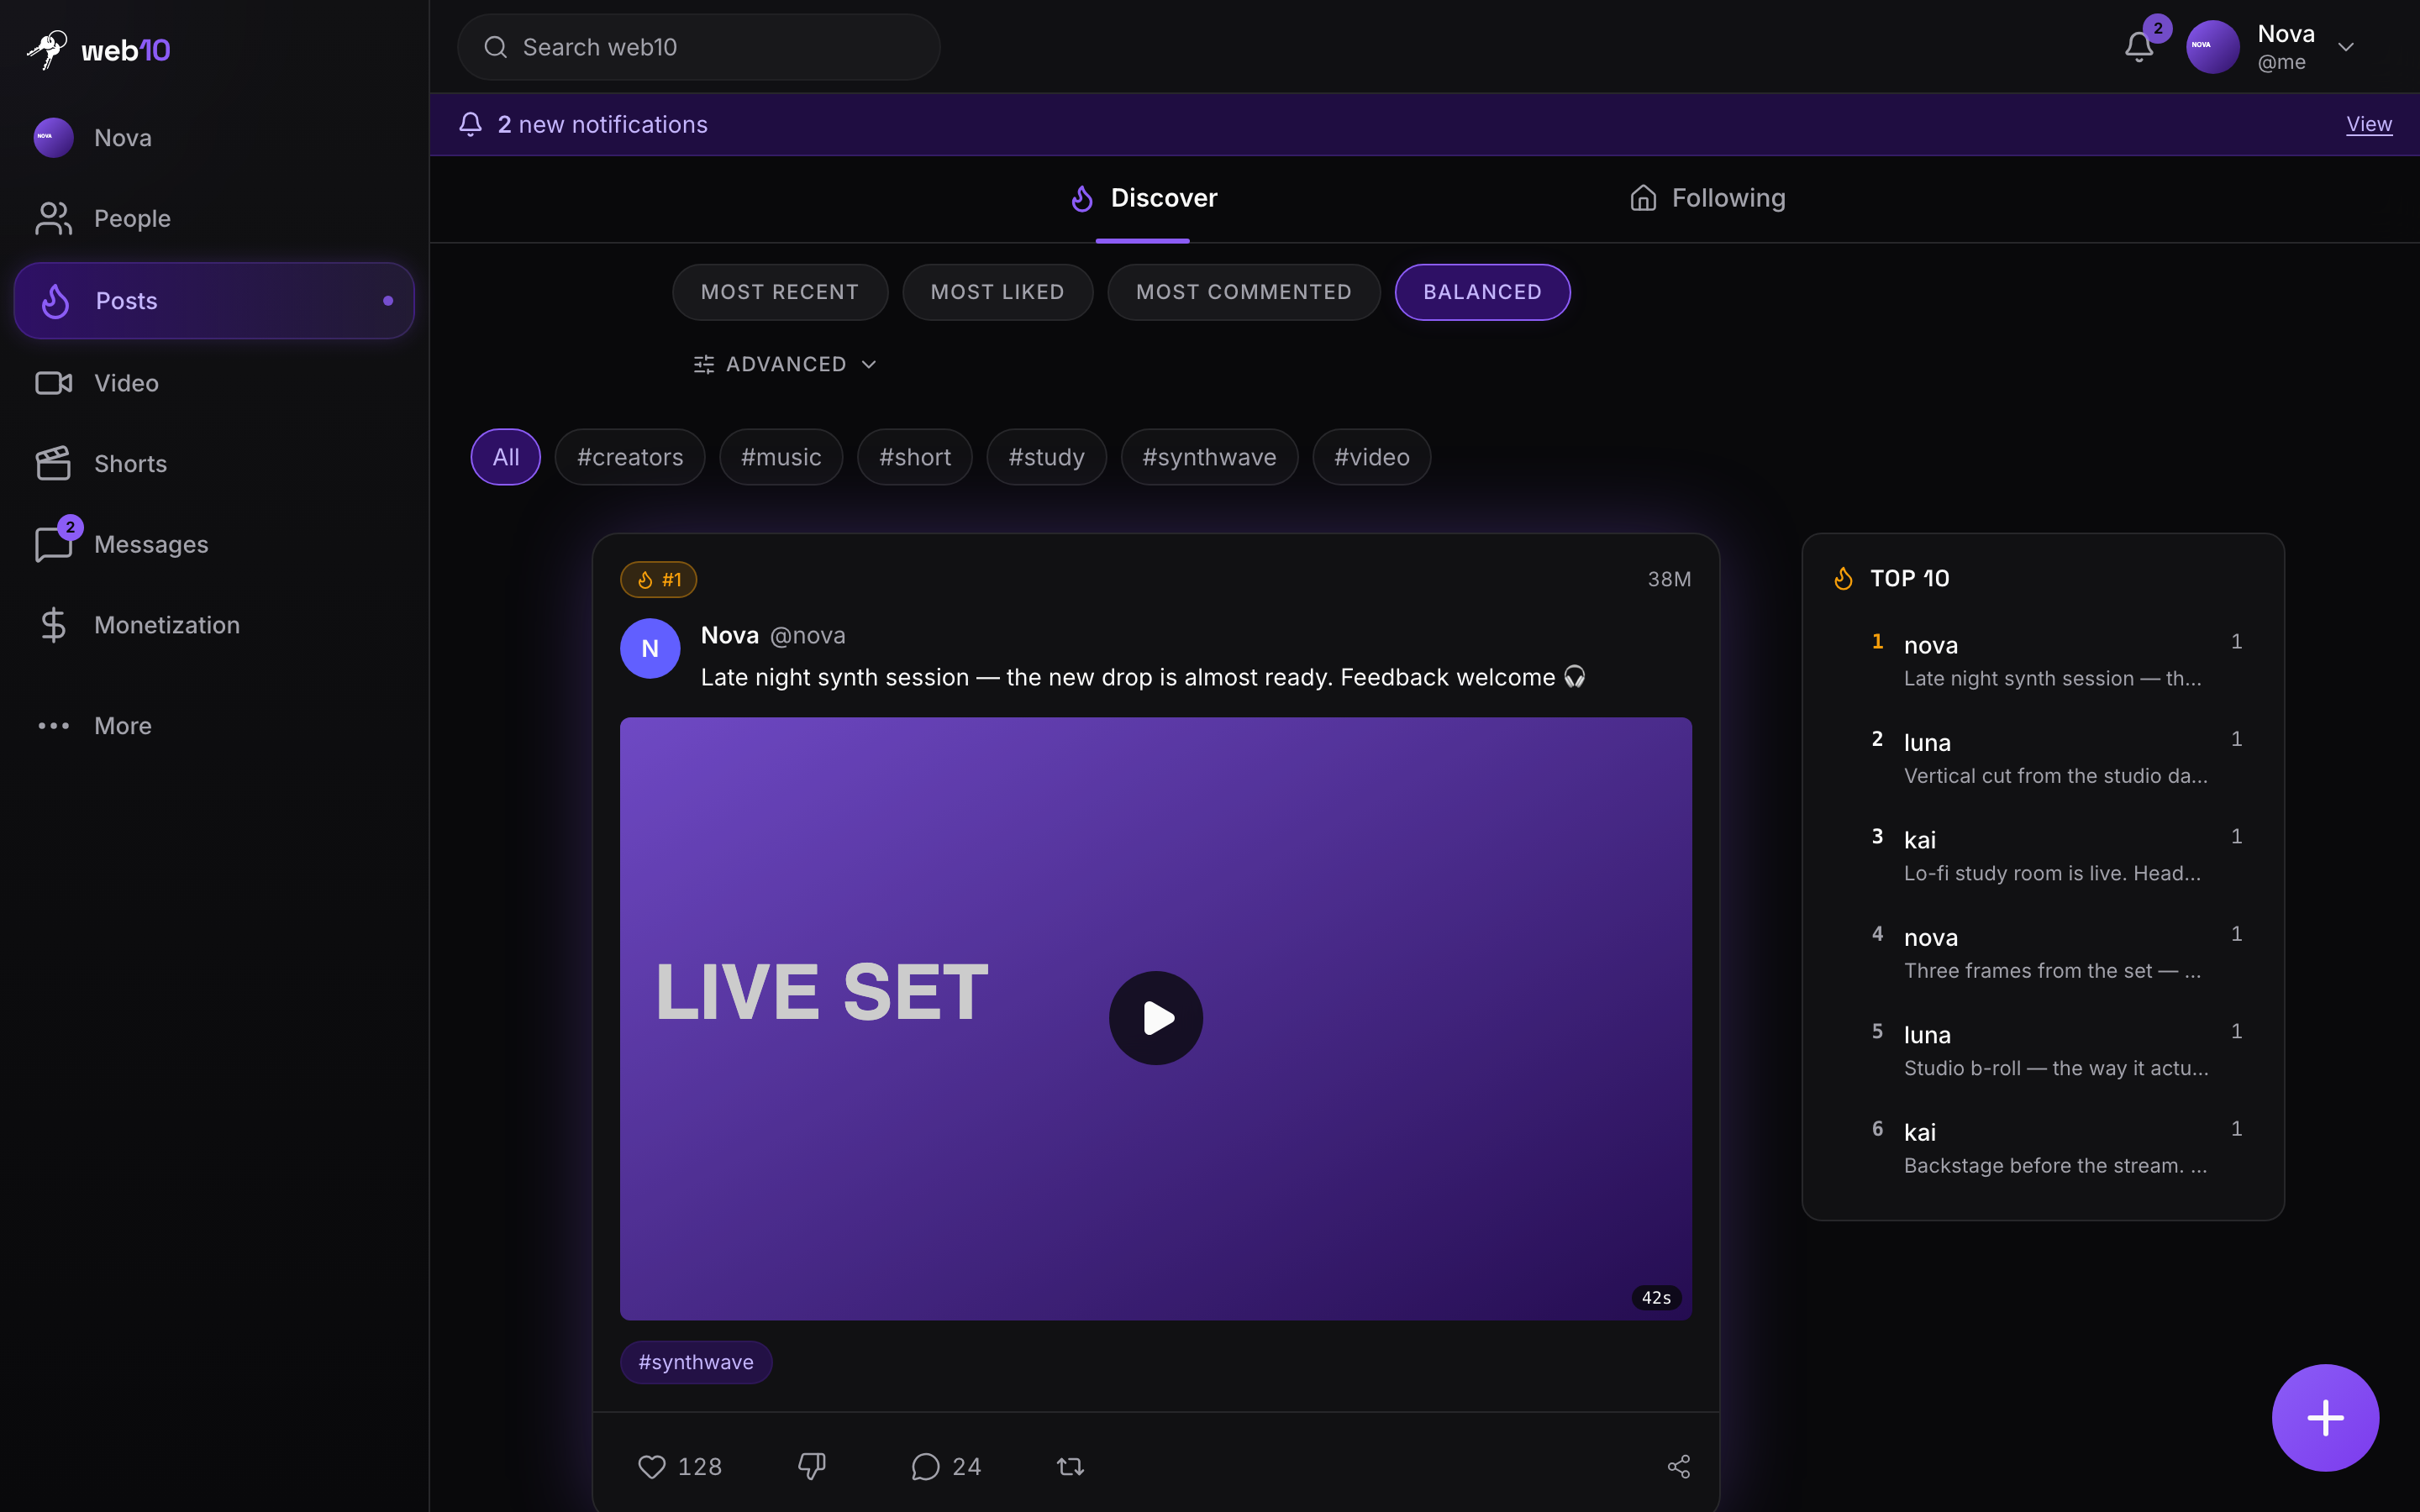
\includegraphics[width=\columnwidth]{figs/fig-feed.png}
  \caption{The web10 feed. The reader chooses the ranking (Most Recent / Most
  Liked / Most Commented / Balanced) and filters (tags); each is a different
  application query over the same columnar store. The main query uses
  reader-specific service boundaries; engagement and view metrics also use
  follow-up calls.}
  \label{fig:feed}
\end{figure}

\begin{figure}[t]
  \centering
  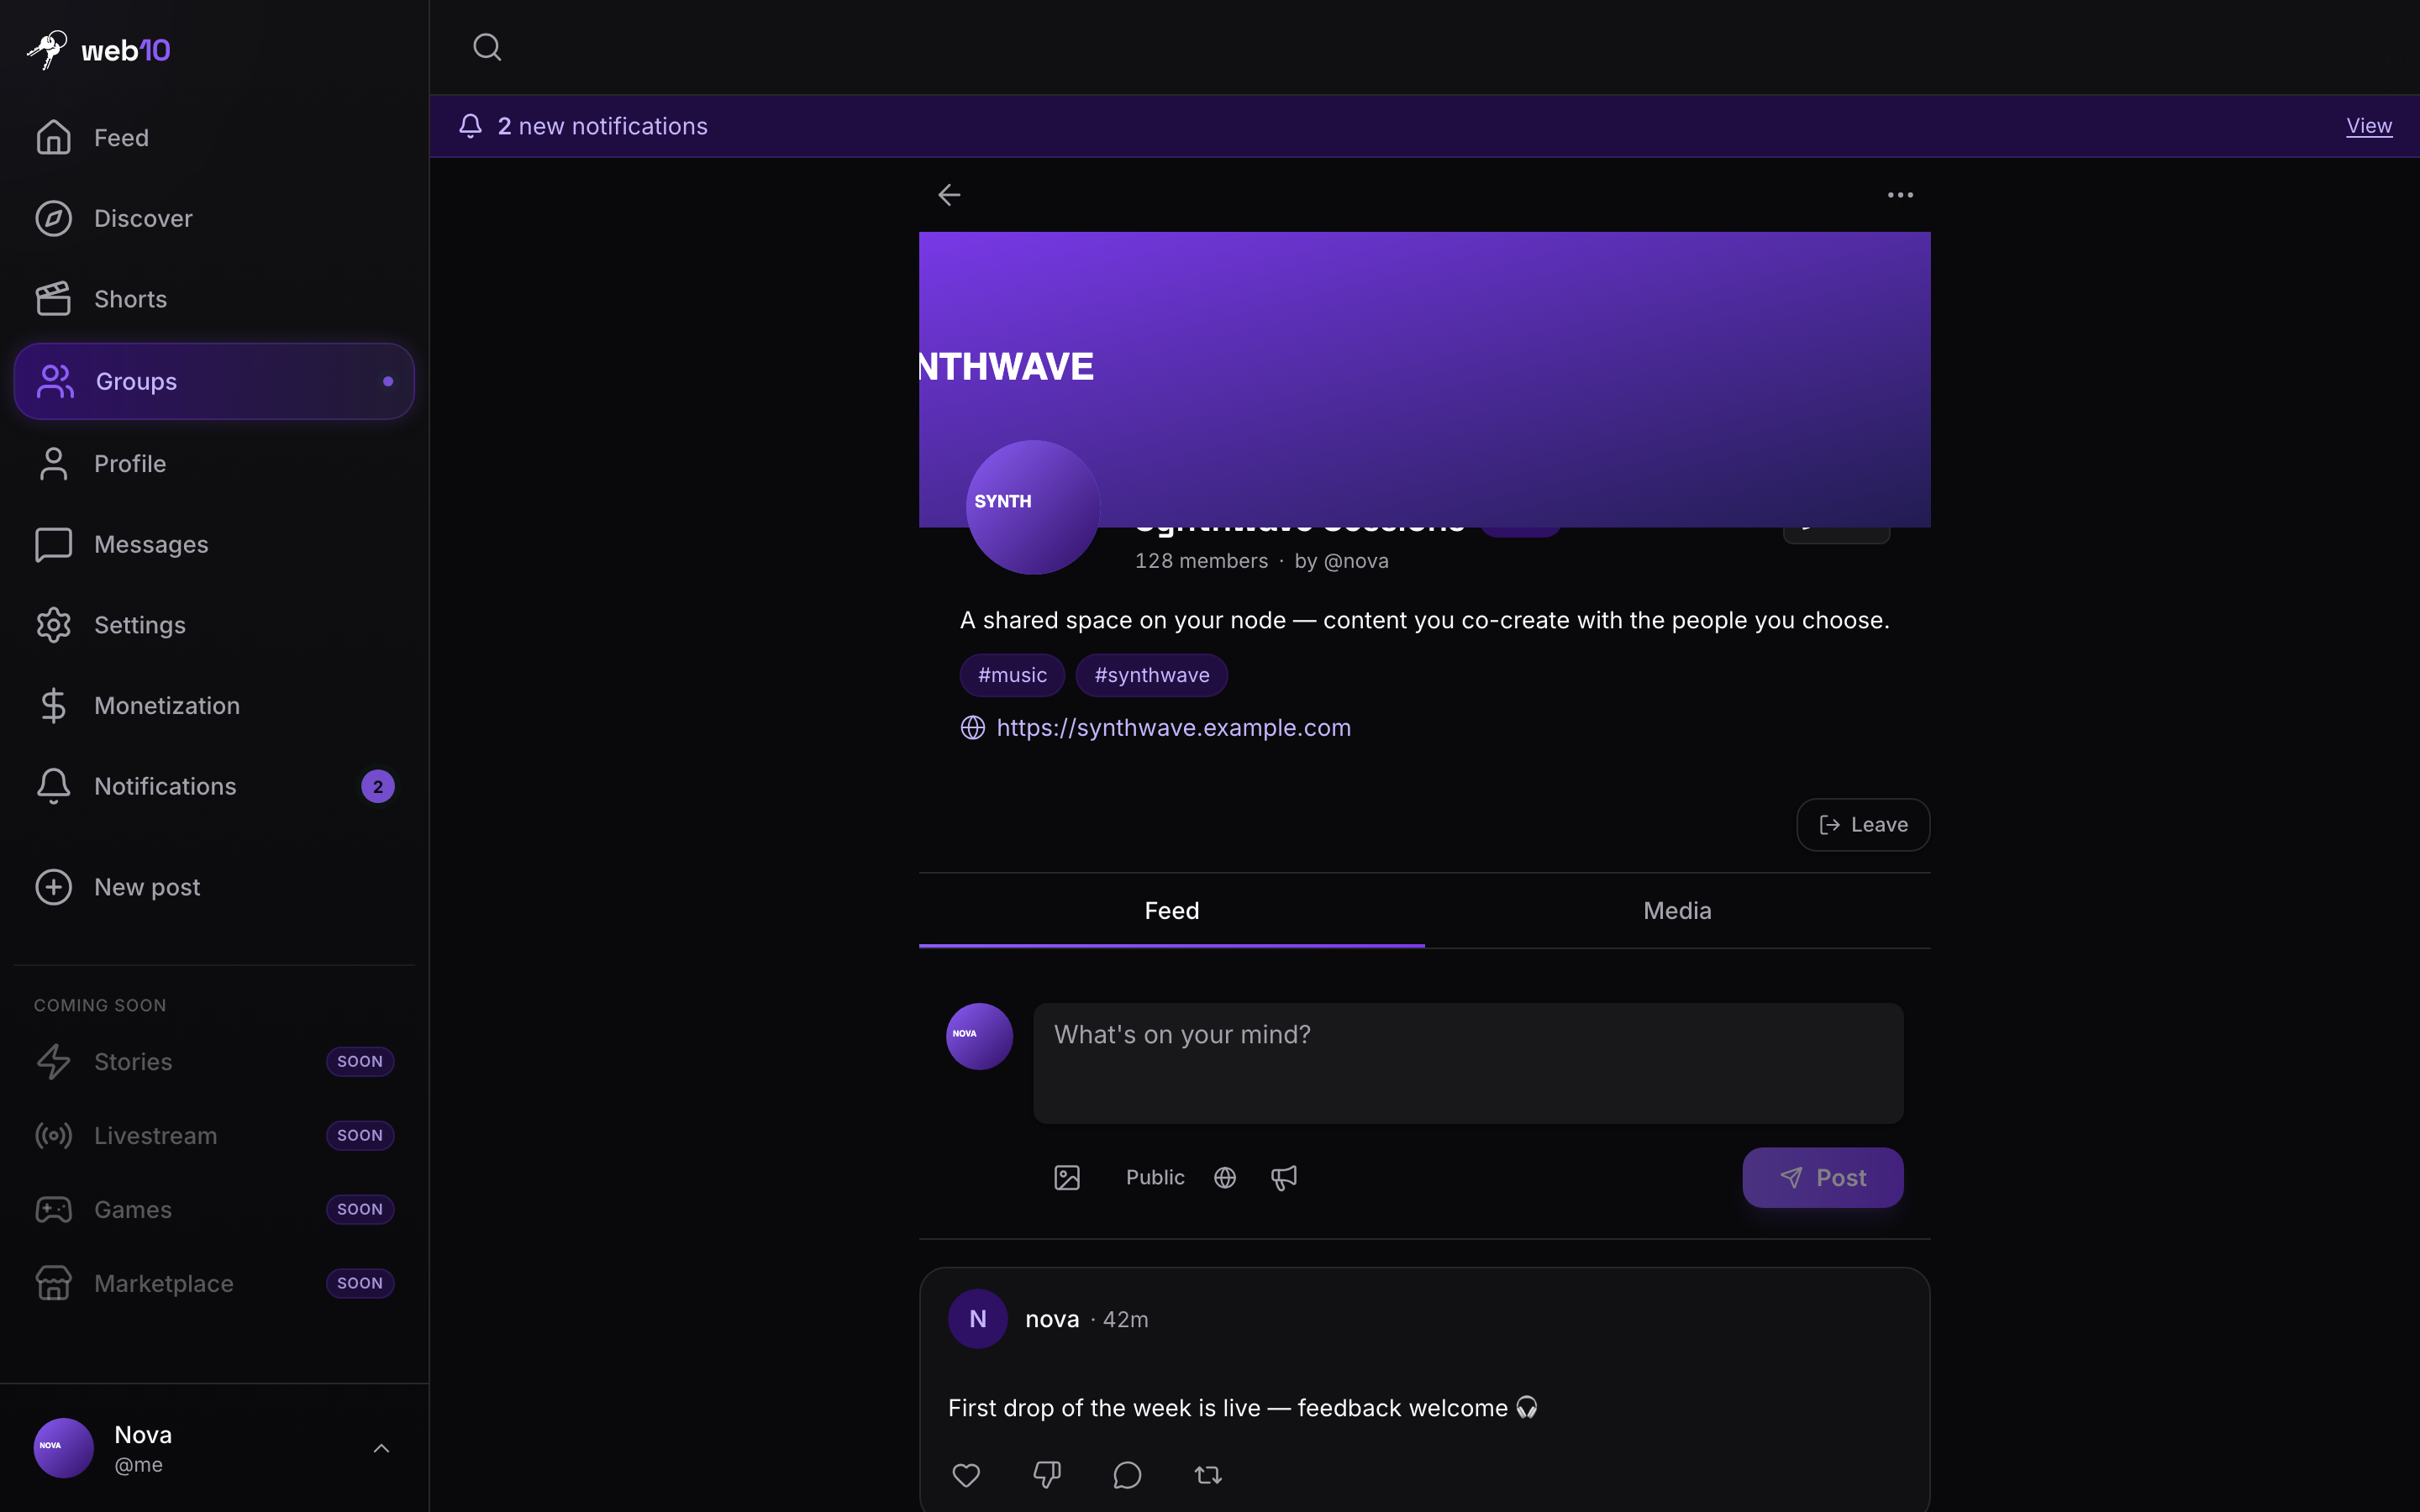
\includegraphics[width=\columnwidth]{figs/fig-groups.png}
  \caption{A group---``a shared space on your node.'' Membership, roles, and
  per-post visibility (Public / node / group) expose application choices over
  the generic groups and grants of \S\ref{sec:model}.}
  \label{fig:groups}
\end{figure}

\subsection{Durability and extensibility}

Application-named services let different clients interpret documents without
changing the shared document schema. A conversation can be a group with message
documents; a music library can define track services and listener roles; a
shop can define catalog services. These are compositional possibilities, not
evidence that every application's requirements fit unchanged. Transactions,
payment workflows, search indexes, schema evolution, and external integrations
may still require additional machinery.

The durable separation is between stored content/access relationships and a
particular frontend. Replacing a frontend can reuse those primitives when it
understands their semantics. Moving providers is a larger task: identity
continuity, document references, group grants, media, and remote relationships
must survive export/import. This paper does not demonstrate complete migration
or federation, and a single-node relational query should not be interpreted as
a cross-node query protocol.

%=============================================================================
\section{Evaluation Status and Methodology}
\label{sec:method}

\subsection{Evidence available and pending}

The evidence here is the implemented architecture, repository tests for named
paths, and a deployed motivating application. The repository includes a
deterministic synthetic-data/load harness and query-phase telemetry. Their
existence is not a completed experiment. This draft has no verified production
scale snapshot, latency distribution, saturation curve, recovery measurement,
or matched baseline result. Empirical evaluation remains pending; neither
commercial capacity nor comparative superiority follows from the screenshots.
Commercial use is the motivation, and measurable service behavior is the bar.

An industry evaluation needs dated production observations separated from
synthetic runs. Production observations should identify deployment duration,
registered and active users, live and versioned document counts, services,
groups, membership distributions, object volume, and operation rates. Counts
of logical user namespaces must not be presented as physical databases. Any
availability, recovery, or operating-cost claim needs its own observation
window, failure definition, and accounting boundary.

\subsection{Workloads and measurement}

Experiments should pin the source revision, dependency and engine versions,
schema, data generator and seed, hardware, storage, network placement, worker
counts, connection limits, and database settings. A localhost harness excludes
wide-area latency but still includes scheduling, queueing, container networking,
and service waits; it is not a browser experience measurement. Browser traces
must separately capture group discovery, main and follow-up queries, media
fetches, and time to a defined render milestone.

Vary document count, versions per document, groups per reader, services per
query, group overlap, response size, ranking complexity, and concurrent writes.
Include member, public-class, authenticated-class, denied, and anonymous reads,
as well as posting, direct-message, and group flows. Multi-group attachments
need explicit duplicate/counting semantics. State warm-up, cache conditions,
run length, offered-load model, concurrency, repeated runs, and uncertainty.
Report successful throughput, errors and timeouts alongside end-to-end
p50/p95/p99 latency; a latency distribution of successful requests alone can
hide overload. Separate API and ClickHouse CPU/memory, storage growth, merge
activity, internal query counts, and resource cost.

The query telemetry times authentication, app contracts, parsing/validation,
candidate discovery, readable-group resolution, group metadata, compilation,
execution, serialization, preparation, and total handler duration. Phase wall
times include waits and do not directly measure Python CPU. The ratio of the
median readable-group phase to median execution time is a descriptive ratio,
not total authorization overhead: policy also changes compilation and the SQL
executed, and ratios of medians are not distributions of per-request overhead.
Instrumentation coverage, including work outside named phases, must be stated.

\subsection{Baselines and correctness}

A conventional shared-table backend with dynamic PostgreSQL RLS is a feasible
baseline~\cite{postgres-rls}, not an intentionally weaker access model. Match
returned content, membership/class grants, visibility exclusions, ranking,
pagination, preparation, consistency requirements, and hardware/resource
budgets. Document indexes, caching, batching, and implementation differences.
Compare full flows as well as database queries. Since web10 already uses a
shared table, the comparison is not ``per-user databases versus shared RLS.''

An authorization-disabled ablation may isolate some costs on synthetic data in
an isolated environment, but is not a functionally equivalent product baseline.
It must account for both metadata orchestration and changes to generated query
plans. Distributed Pod or federated architectures offer different placement
and autonomy properties; any comparison must describe those tradeoffs rather
than infer inferior performance from topology alone.

Correctness evaluation should publish a pinned test matrix and actual results,
distinguishing unit tests, mocked endpoints, and live-store and browser tests. Cover
principal classes, membership admission, service permissions, tombstones,
multi-group rows, aggregations, nested SQL, denied raw tables/functions, and
capability issuance. Revocation experiments must race grant changes with reads
and measure stale access through metadata visibility, in-flight requests, and
issued URLs/manifests. Current security work retains unresolved credential,
consent/delegation, and media-boundary questions; regression tests on selected
query paths do not close them. The paper requires measured outcomes and bounded
coverage statements, not a blanket security label or a promised later report.

%=============================================================================
\section{Related Work}
\label{sec:related}

\textbf{Decentralized social data.} ActivityPub~\cite{activitypub2018} defines
client/server and federated server/server activity delivery. ATProto's
repositories, relays, and AppViews separate storage from application views and
support user agency and provider switching~\cite{kleppmann2024}. web10 focuses
on query composition within a node: app-defined service queries read a shared
store through relations filtered for the reader at request time. Federation
and provider migration address complementary system boundaries.

Solid separates applications from personal data stores~\cite{solid2016}, with
social application work~\cite{solid-apps2016} and a maintained Community Solid
Server~\cite{css2024}. WAC supports resource permissions and group agents
through \texttt{acl:agentGroup}~\cite{wac2022}; ACP includes agent, client, and
issuer matching~\cite{acp2022}. web10 packages group membership,
join policies, and per-service role maps with a shared relational query path.
Pods are logical stores that need not each occupy a separate server; cross-store
query cost depends on deployment, caching, indexing, and query strategy. The
comparison here concerns data placement and query interfaces; a performance
comparison would require a matched workload and deployment.

\textbf{Cloud IAM.} AWS IAM (documentation)~\cite{awsiam} and the
RBAC/ABAC literature~\cite{ferraiolo1992, sandhu1996, abac2014} provide the
policy concepts web10 adapts at the user boundary: principals, roles,
service-scoped operations, revocable grants. The move in this paper is
directional---a familiar policy vocabulary exposed to users about their own
content and groups, orchestrated by the API and query layer. At industrial
scale, relationship-based authorization (Zanzibar~\cite{zanzibar2019}) shows
a uniform ACL data model and consistency as a first-class problem. Its
consistency guarantees motivate explicit evaluation of web10's revocation
visibility. TAO~\cite{tao2013} provides a social-graph storage precedent, whereas
web10 composes application queries over service-namespaced documents in a
columnar store.

\textbf{Multi-tenant isolation.} The database literature on tenant
isolation---shared tables with an organization identifier
(Force.com~\cite{force2009}), schema-mapping techniques
~\cite{aulbach2008}, and the shared-versus-separate spectrum
~\cite{jacobs2007}---is the closest systems ancestor. web10's key-space per
user makes the \emph{end user} the logical tenant. Authorship uses
\texttt{author\_key}; shared reads use authorized group relations rather than
a physical database boundary.
PostgreSQL row-security policies~\cite{postgres-rls} are an alternative location
for dynamic access enforcement. Matched policy and workload execution
(\S\ref{sec:method}) can distinguish the costs of these enforcement placements.
ClickHouse~\cite{clickhouse2024}
supplies the columnar execution engine; web10 supplies the access orchestration
above it, including metadata resolution, SQL compilation, and result preparation.

%=============================================================================
\section{Conclusion}
\label{sec:concl}

web10 makes content and access relationships a shared substrate for application
queries. Logical user namespaces, app contracts, and generic groups connect
user-managed access to a columnar store; the query layer supplies the reader's
service relations before joins and aggregation. The social application shows
how this separation supports ranked feeds and scoped engagement reads while
keeping query definitions in the application.

The next step is to establish a practical operating point and characterize
metadata fan-out, query execution, and revocation under representative workloads.
Those measurements remain pending. They will provide a baseline for subsequent
optimization of policy resolution and query processing. The architectural
contribution is this integration: applications compose social views over
reader-specific service relations in a shared columnar store.

%=============================================================================
\bibliographystyle{ACM-Reference-Format}
\bibliography{../references/web10-references}

\end{document}
